\chapter{Experimental Apparatus}
\label{chap:Detector}
\textcolor{red}{\bf \large {Introduction}}
The LHC is to reveal the physics beyond the Standard Model with centre-of-mass collision energies up to 14 TeV and luminosity up to 10$^{34}$ cm$^{-2}$s$^{-1}$. At present, the center-of-mass energy at the LHC is at 8 TeV and it will increase to around 14 TeV collision energy by around 2015. Due to the availability of very high energy for the collisions, it becomes possible for the researchers to understand the fundamental structure of the universe deeply and to look back in its history. 

\section{The Large Hadron Collider}
The Large Hadron Collider (LHC) \cite{Evans:2008zzb} is the world's biggest and the most powerful particle accelerator and collider built by CERN (European Organization for Nuclear Research), at Geneva, Switzerland. It occupies the 27 km circumference circular tunnel (between the border of France and Switzerland), previously used by LEP (Large Electron-Positron) collider \cite{LEP}, at a depth ranging from 50 to 175 metres (164 to 574 ft) underground. Two beams of particles of the same kind, either protons or lead or xenon ions, are accelerated in direction opposite to each other. 1,232 dipole magnets maintain the beams in their circular path and 392 quadrupole magnets keep the beams focused to increase the probabilities of interaction between the particles. Since this thesis is based on the proton-proton (pp) collisions data, the main focus is on protons. 

The protons pass through a series of accelerators which increase their energy successively before their injection into the main ring of LHC. Figure~\ref{fig:LHC} gives an overview of the various accelerators and detectors comprising the complex structure of the LHC. The protons are obtained by stripping of electrons from hydrogen gas atoms using an electric field. The protons are accelerated up to 100 keV through a radiofrequency quadrupole which provides the first focusing and a further acceleration to 750 keV energy. The linear particle acclerator (LINAC2) increases the energy of protons to 50 MeV. Then these protons are injected into the Proton Synchrotron Booster (PSB) in the form of bunches where they get accelerated to 1.4 GeV energy. The energy of protons is further enhanced to 25 GeV by Proton Synchrotron (PS) and then to 450 GeV by the Super Proton Synchrotron (SPS). Finally the protons are injected into two beam pipelines of the main LHC ring where their energy increases to the collision energy. 

The accelerated beams are made to collide at four interaction points around which six detectors : ALICE (A Large Ion Collider Experiment) \cite{Aamodt:2008zz}, ATLAS (A Toroidal LHC Apparatus) \cite{Aad:2008zzm},  CMS (Compact Muon Solenoid) \cite{Chatrchyan:2008aa,Bayatian:2006nff,Ball:2007zza}, LHCb (Large Hadron Collider for Beauty) \cite{Alves:2008zz}, LHCf (Large Hadron Collider forward)\cite{Adriani:2008zz} and TOTEM (ToTal Elastic and diffractive cross section Measurement) \cite{Anelli:2008zza}, are located. The CMS and ATLAS are the two general purpose detectors dedicated to the search of the Higgs boson, existence of super-symmetry (SUSY) and also looking for extra dimensions. The ALICE is a heavy-ion detector which collides lead ions to study quark-gluon plasma, a state of matter believed to be present just after the Big Bang. The LHCb experiment will explore the differences between matter and antimatter and new physics through b-quark (beauty) studies. TOTEM experiment is dedicated to cross section measurements whereas LHCf focuses on forward physics  The LHC operated at the centre-of-mass energy (\cme) of 7 TeV of pp collisions in the 2010 and 2011 and at \cme = 8 TeV in the year 2012. After the upgradations , it restarted in 2015 at a much higher centre-of-mass energy of 13 TeV and is running successfully till now. In the coming years, protons will be made to collide at a designed \cme = 14 TeV with luminosity up to 10$^{34}$ cm$^{-2}$s$^{-1}$. In this thesis, work has been carried out using the pp collisions data collected by the CMS detector at \cme = 8 TeV.

\begin{figure}[!h]
 \begin{center} 
 \hspace*{-5mm}
 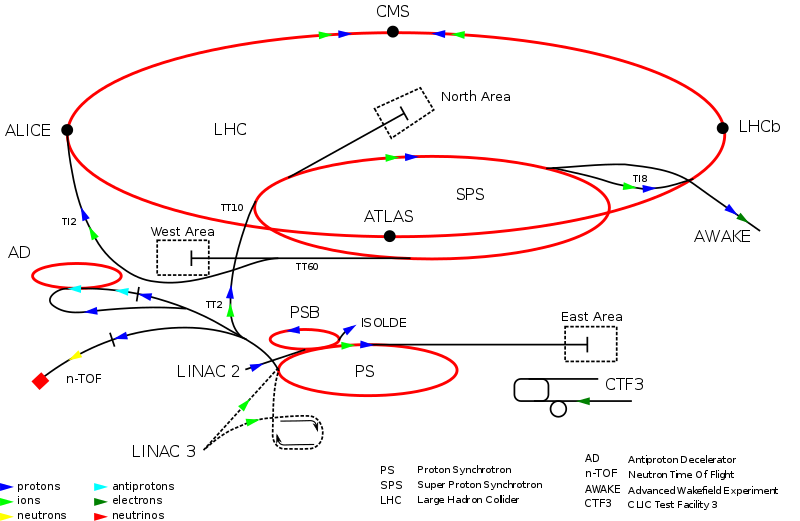
\includegraphics[width=1.\textwidth]{/home/anter/Desktop/Thesis/Figures/LHC.png}\\
 \vspace*{5mm}
 \caption[LHC]{Overview of the different experiments of the Large Hadron Collider (LHC), a complex particle accelerator and collider located at CERN.\footnotemark}
 \label{fig:LHC}
 \end{center}
\end{figure}
\footnotetext{Source : \url{http://public.web.cern.ch/public/en/research/AccelComplex-en.html}}

\section{Luminosity Measurement}
Luminosity (\lumi) is one of the most important parameters of an accelerator which characterizes its performance. It gives the rate at which collisions occur and given by the number of collisions produced in a detector per cm$^2$ and per second. Cross section ($\sigma$) is a measurement of the probability that an event occurs. It is related to total number of events $N$ of a process over a time period T and \lumi as :
\begin{equation}
N = \int_{0}^{T} \lumi~\sigma~dt = \lumi_{int}~\sigma
\end{equation}
where $\int_{0}^{T} \lumi~dt = \lumi_{int}$ is the total integrated luminosity. It is usually expressed in units of barn$^{-1}$ and gives a direct indication of the number of produced events for a process. For example, an integrated luminosity of 10 fb$^{-1}$ means that 10 events are produced in a process with cross section equal to 1 fb.

The luminosity depends on the particle beam parameters and is given by :

\begin{equation}
\lumi = \frac{N^2_p~N_b~f_{rev}~\gamma~F}{4\pi~\epsilon_n~\beta^*}
\end{equation}
where $N_p$ is the number of particles per bunch, $N_b$ is the number of bunches per beam, $f_{rev}$ is the revolution frequency of the beam, $\gamma$ is the relativistic gamma factor and $F$ gives the geometric luminosity reduction factor. The effective collision area of the two beams is related to the normalized transverse beam emittance $\epsilon_n$ and the value of the betatron function $ \beta^*$ at the interaction point.
 
The CMS experiment constantly monitors the instantaneous luminosity delivered by LHC which is shown versus time in Fig.~\ref{fig:lumi} for proton-proton collisions at nominal center-of-mass energy for the years 2010-2017. The relative instantaneous luminosity is calculated by using two methods \cite{CMS:2013gfa} : Hadron Forward (HF) method by measuring the particle flux in the hadron forward calorimeter and by counting the number of reconstructed vertices in the pixel tracker. The absolute luminosity measurement relys on van-der-Meer scans done in special runs of the LHC \cite{vanderMeer:1968zz}. The uncertainty on the luminosity measured for 2012 data set is 2.5\% (syst.) and 0.5\% (stat.).

\begin{figure}[!h]
 \begin{center}
 \vspace*{4mm} 
 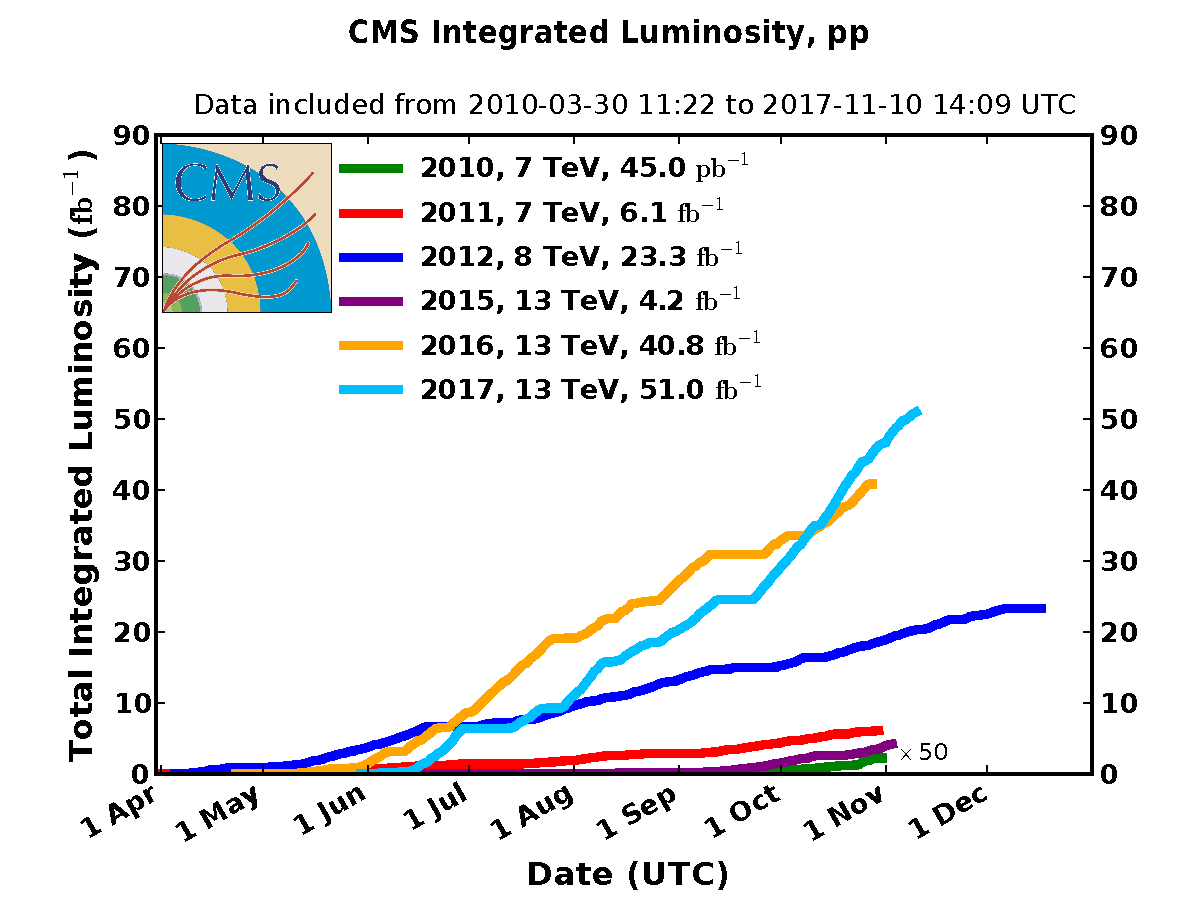
\includegraphics[width=.8\textwidth]{/home/anter/Desktop/Thesis/Figures/int_lumi_cumulative_pp_2.pdf}\\
 \vspace*{5mm}
 \caption[Lumi]{The integrated luminosity, delivered to CMS during stable beams for proton-proton collisions at nominal center-of-mass energy, is shown versus time for data-taking in 2010 (green), 2011 (red), 2012 (blue), 2015 (purple), 2016 (orange) and 2017 (light blue) run periods of the LHC.\footnotemark}
 \label{fig:lumi}
 \end{center}
\end{figure}

\section{The Compact Muon Solenoid}

\footnotetext{Source : \url{https://twiki.cern.ch/twiki/bin/view/CMSPublic/LumiPublicResults}}
The Compact Muon Solenoid (CMS) detector is a general purpose detector located at the interaction point 5 (P5) of the main LHC ring, near the village of Cessy in France. The name of CMS comes from its compact size with main emphasis on the detection of muons and enclosed within high solenoidal magnetic field. The CMS detector aims at identifying the different types of particles produced in proton-proton and heavy ion collisions and measuring their energies and momenta. This is achieved by layers of different sub-detectors arranged in a cylindrical complex structure with 21.6 m length and 15 m diameter. The silcon-based tracker suurounds the the interaction point and forms the innermost layer. It is surrounded by a scintillating crystal electromagnetic calorimeter (ECAL) and a sampling hadron calorimeter (HCAL) which are enclosed inside the superconducting solenoid. Outside the magnet lies the large muon detectors embedded inside  an iron yoke. The three dimensional view of the CMS detector along with its components is presented in Fig.~\ref{fig:CMS}. The CMS was constructed in parts at ground and assembled later on in the cavern. The components are easily accessible for upgrades or repairs as the detector can be opened up into movable slices. Figure~\ref{fig:CMS_front} shows the front view of the CMS detector differentiating individual components which contribute to event reconstruction. The path of reconstructed particles is represented by dashed (invisible track) and solid (visible track) lines for different particle classes : photons ($\gamma$), muons ($\mu^{\pm}$), electrons (e$^{-}$), neutrons (n) and charged hadrons (pions $\pi^{\pm}$).
\begin{figure}[!h]
\begin{center}
\vspace{2mm}
\hspace*{-10mm}
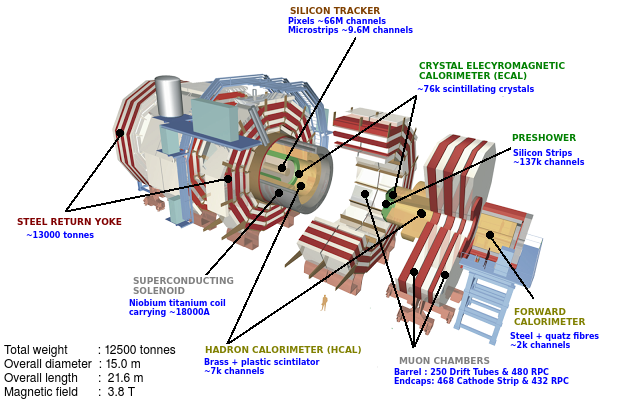
\includegraphics[scale = 0.98]{/home/anter/Desktop/Thesis/Figures/CMS_2_new.png}\\
\vspace*{5mm}
\caption[CMS]{The three dimensional view of the CMS detector along with its sub-detector components.\footnotemark}
\label{fig:CMS}
\end{center}
\end{figure}
\footnotetext{Source : \url{https://orbiterchspacenews.blogspot.in/2013/04/cern-cms-prepares-for-future.html}}

\begin{figure}[!h]
\begin{center} 
\hspace*{-15mm}
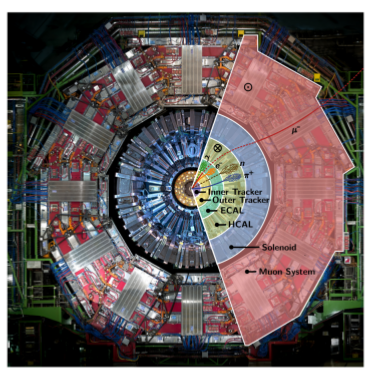
\includegraphics[scale = 0.75]{/home/anter/Desktop/Thesis/Figures/CMS_Front_2.png}
\caption{Front view of the CMS detector \cite{Ball:2007zza} along with its components : inner tracker, outer tracker, electromagnetic calorimeter, hadronic calorimeter, solenoid and muon system. The path of different particles detected by dedicated sub-detectors are shown by dashed (invisible track) and solid (visible track) lines. $\otimes$ and $\odot$ gives the direction of magnetic field inside the solenoid and in the return yoke, respectively.}
\label{fig:CMS_front}
\end{center}
\end{figure}

A brief overview of the CMS detector has been presented and the details of the its design as well as physics performance are available in Ref.~\cite{Bayatian:2006nff,Ball:2007zza}. Before going into the details of each sub-detector, first we described the coordinate system used by CMS in the next section.

\subsection{Coordinate System}
CMS uses right-handed coordinate system having origin at the nominal interaction point of the collision inside the detector. The $x$-axis points horizontally towards the center of the LHC ring, the $y$-axis vertically upwards and the $z$-axis along the beam direction towards the Jura mountains. Following customary polar coordinate conventions, the
azimuthal angle $\phi$ is measured from the x-axis in the x-y plane as $\phi = {\rm tan^{-1}}(\frac{y}{x})$, and the polar angle $\theta$, from the z-axis in the z-y plane as $\theta~=~{\rm tan^{-1}}\big(\frac{x^2~\plus y^2}{2}\big)$. The quantities pseudorapidity $\eta$ and the rapidity $y$ are preferred over the angles $\theta$ and $\phi$. The pseudorapidity and rapidity are given by Eq.~\ref{eq:pseudorap}. Both the quantities are equal for massless particles.

\begin{equation}
\begin{gathered}
\eta = -~{\rm ln}\bigg({\rm tan}\bigg(\frac{\theta}{2}\bigg)\bigg)\\
y = \frac{1}{2}~{\rm ln} \bigg(\frac{E~\plus p_z}{E - p_z} \bigg)
\end{gathered}
\label{eq:pseudorap}
\end{equation}
The difference between rapidities $\Delta y$ is invariant under longitudinal Lorentz boost whereas it does not hold for $\eta$. Hence $y$ is considered in this thesis. The angular distance between the two particles is defined by $\Delta R = \sqrt{(\Delta \eta)^2~\plus (\Delta \phi)^2}$. The momentum component transverse to the direction of beam \pt, is computed from the $x$- and $y$-components as \pt = $\sqrt{p^2_x~\plus p^2_y}$ and the transverse energy is given by $E_T$ = $E$ sin $\theta$.
 
\subsection{Inner Tracker System}

\begin{figure}[!h]
\begin{center} 
\hspace*{-15mm}
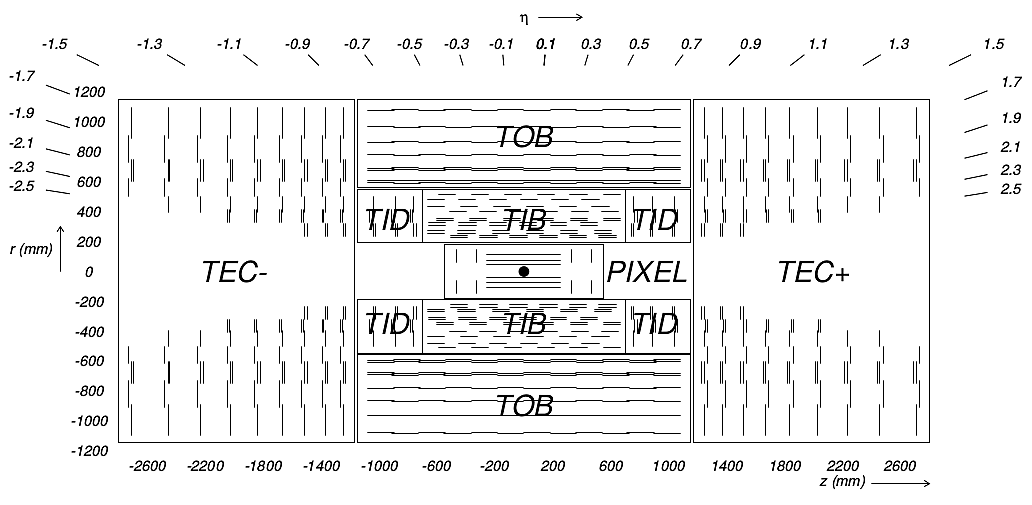
\includegraphics[scale = 0.75]{/home/anter/Desktop/Thesis/Figures/Tracker.png}
\caption{A schematic diagram of tracker in CMS experiment \cite{Chatrchyan:2008aa}. The figure shows
two quadrants of a longitudinal section of the inner tracking detector of CMS along r-z
plane. The strip detector comprises four components: The Tracker Inner Barrel (TIB)
is complemented by the Tracker Inner Disks (TID). These two are surrounded by the
Tracker Outer Barrel (TOB). High $\eta$ ranges are covered by the Tracker End Cap (TEC)
up to $\eta$ = 2.5}
\label{fig:Trcaker}
\end{center}
\end{figure}

\subsection{Electromagnetic Calorimeter}

\subsection{Hadron Calorimeter}

\subsection{Superconducting Magnet}

\subsection{Muon System}

\subsection{Trigger system}

\section{Computing and Software Tools}

\subsection{Analysis Software}

\subsection{Monte Carlo Event Generators and Simulation Software}

\section{Reconstruction of Jets} 
\begin{comment}

 \begin{itemize}
\item
\textbf{Inner Tracking System :} The charged particles produced from the LHC collisions leave their trajectories as they move outward from the interaction point. These trajectories are measured precisely and efficiently by the inner tracking system of CMS. The inner tracking system also reconstructs secondary vertices. It surrounds the interaction point and has a cylindrical volume of length of 5.8 m and a diameter of 2.5 m. A pixel detector with three barrel layers at radii between 4.4 cm and 10.2 cm and a silicon strip tracker with 10 barrel detection layers extending outwards to a radius of 1.1 m are the integral parts of the tracking system. Two disks form the endcaps in the pixel detector whereas 3 plus 9 disks on each side of the barrel completes the strip tracker on its end. These endcaps extend the acceptance of the tracker up to a pseudorapidity of $|\eta| < 2.5$ ($\eta$ = $-$ log tan($\frac{\theta}{2}$), where $\theta$ is the angle between particle momentum and beam direction). The active silicon area of CMS tracker is about 200m$^{2}$ which makes it the largest silicon tracker. There are calorimeters outside the tracker to measure the energy of particles. The tracker should interfere with the particles to a minimum extent so that their momentum can be measured precisely. To measure their energy, they are required to interact with the calorimeters fully.
 \item
\textbf{Electromagnetic Calorimeter :} The electromagnetic calorimeter (ECAL)~\cite{ecal} consists of an array of lead tungstate (PbWO$_{4}$) crystals with coverage in pseudorapidity up-to $|\eta| <$ 3.0. The produced photons and electrons interact with matter mainly through bremsstrahlung and electron-positron pair production and deposit most of their energy in calorimeter. The deposited energy is converted to scintillation light which is detected by silicon avalanche photo diodes (APDs) in the barrel region and vacuum phototriodes (VPT) in the end-cap region. The number of created photons gives the direct measure of energy of the incident particle. Also, the pre-shower detectors made of lead absorbers and silicon detectors are put in front of the endcaps to distinguish high energetic single photons from low energetic photon pairs originating from $\pi^{0}$ decays. 

\item
\textbf{Hadron Calorimeter :} The Hadron Calorimeter (HCAL)~\cite{hcal} is designed to detect any particle made up of quarks (the basic building blocks of protons and neutrons) and measurement of hadron jets and neutrinos or exotic particles resulting in apparent missing transverse energy. The region between the outer extent of the electromagnetic calorimeter (R = 1.77 m) and the inner extent of the magnet coil (R = 2.95 m) encloses the hadron calorimeter barrel (HB). The total amount of material in this region to absorb the hadronic shower is not sufficient. This requirement is fulfilled by placing an outer hadron (HO) calorimeter or tail catcher outside the solenoid. The forward hadron calorimeter (HF) placed at 11.2 m from the interaction point covers the pseudorapidity, 3.0 < $|\eta|$ < 5.2. Hadronic barrel (HB) and hadronic endcap (HE) calorimeters are sampling calorimeters made up of 50mm thick copper (selected because of its density) absorber plates interleaved with 4mm scintillator sheets. HB is made of two 4.4m length half-barrels, and HE has two large structures, situated at each end of the barrel detector and within the region of high magnetic field.  HF, situated at each extreme of the CMS detector, is made of steel absorbing plates along with quartz fibers. The passage of charged particles through the quartz fibers produces Cerenkov light signals, which are used to measure the energy of the jets. 

 \item
\textbf{The Superconducting magnet :} The Superconducting magnet is 13m long and 6m in diameter. Its refrigerated superconducting niobium-titanium coils are cooled at -270$^{\circ}$C to produce a magnetic field of 4 Teslas. This intense solenoidal field makes the compactness and cylindrical symmetry of the detector possible. The tracker and calorimeters are placed inside the magnet making the detector compact in size. The solenoidal magnetic field parallel to the beam bends the tracks of the charged particles in the transverse plane. The curvature of these tracks gives the measurement of momentum.

\item
\textbf{Muon System :} As the name suggests, the detection of muons is of central importance to CMS. The muon system has three functions: muon identification, momentum measurement and triggering. Good muon momentum resolution and trigger capability are enabled by the high-field solenoidal magnet and its flux-return yoke. The latter also serves as a hadron absorber for the identification of muons. The CMS muon system is designed to have the capability of reconstructing the momentum and charge of muons over the entire kinematic range of the LHC. There are 3 types of gaseous particle detectors for muon identification : Resistive Plate Chambers (RPC), Cathode Strip Chambers (CSC) and Drift Tubes (DT). The details of all these detectors can be found in~\cite{muon}. RPCs can be operated at high rates and thus provide fast information which is used for the Level-1         trigger.                                                                

\item
\textbf{Trigger system :} The Trigger and Data Acquisition (DAQ) system of an experiment at a hadron collider plays a crucial role. Both the collision and the overall data rates are much higher than the rate at which the information can be stored. The p-p collisions (events) take place at high interaction rates at LHC. An average of 17 events occurs at the beam crossing frequency of 25 ns for the nominal LHC design luminosity of 10$^{34}$ cm$^{-2}$s$^{-1}$. The CMS Trigger and Data Acquisition System (TriDAS) observes the detector information at the full crossing frequency and selects events at a maximum rate of O(10$^{2}$) Hz for archiving and later offline analysis. The required rejection power of O(10$^{5}$) is very large. The high efficiency for the interesting events should also be maintained. These tasks are split into two steps $-$
\begin{itemize}
\item
The Level-1 Trigger~\cite{trigger} : At the first level all data is stored for 3.2 $\mu$s, after which no more than 100 kHz of the stored events are forwarded to the next level triggers. This must be done for all channels without dead time, while full data are stored temporarily in pipeline memories in the the front-end electronics of the sub-detectors. Due to this time restriction and the number of channels and complexity of the reconstruction involved, the central tracking system is not used in the L1 trigger decision. The Level-1 (L1) system is based on custom electronics. The L1 system uses only coarsely segmented data from calorimeter and muon detectors, while holding all the high-resolution data in pipeline memories in the front-end electronics.
\item
The High Level Trigger~\cite{hlt} : The second step, High-Level Trigger (``HLT'') is designed to reduce the maximum Level-1 accept rate of 100 kHz to a final output rate of 100 Hz. The HLT system relies upon commercial processors. The HLT is provided by a subset of the on-line processor farm which, in turn, passes a fraction of the accepted events to the remainder of the on-line farm for more complete processing.

The trigger is the start of the physics event selection process. A decision to retain an event for further consideration has to be made every 25 ns. This decision is based on the event's suitability for inclusion in one of the various data sets to be used for analysis. The data sets to be taken are determined by CMS physics priorities as a whole. These data sets include di-lepton and multi-lepton data sets for top and higgs searches, lepton plus jet data sets for top physics, and inclusive electron data sets for calorimeter calibrations. In addition, other samples are necessary for measuring efficiencies in event selection and studying backgrounds. The trigger has to select these samples in real time along with the main data samples.
\end{itemize}
\end{itemize}
\begin{comment}
\section{CMS Detector}
The aim of a particle detector is to count the particles produced that pass through it after being produced in a collision or a decay - an ``event'', to visualise their tracks, to measure their energies and momenta, to record time-of-flight and to identify their identity. The exact position where the event occurs is known as the interaction point. It is neccessary to know the mass and momentum of the particles to identify them. The mass can be found by measuring either the velocity or the energy and the momentum. Depending on the type of the particles and forces to be studied, various detectors have been designed.

In particle physics, a hermetic detector, also known as a 4$\pi$ detector, is a particle detector which is designed to observe all possible decay products of an interaction between subatomic particles in a collider. It covers a large area around the interaction point and  consists of layers of sub-detectors each specialising in a particular type of particle or property. They are typically cylindrical having different types of detectors wrapped around each other. These are known as hermetic because their construction is such that the motion of particles is ceased at the boundaries of the chamber and the particles donot move beyond the seals. These detectors cover solid angle nearly of 4$\pi$ steradians around the interaction point and hence are named as ``4$\pi$'' detectors.

The first 4$\pi$ detector was the ``Mark I'' at the Stanford Linear Accelerator Center (SLAC) which resulted in the discoveries of J/$\psi$ particle and $\tau$ lepton. Its basic design has been used for all modern collider detectors. Prior to the building of the Mark I, it was thought that most particle decay products would have relatively low transverse momentum (i.e. momentum perpendicular to the beamline), so that detectors could cover this area only. However, it was learnt at the Mark I and subsequent experiments that the most fundamental particle interactions at colliders involve very large exchanges of energy and therefore involve large transverse momenta. So the large angular coverage is taken into account for modern particle physics.

The modern particle large-scale detectors in use in accelerators such as Large hadron collider at CERN which includes ATLAS and LHCb or HERA at DESY are hermetic detectors. The accelerators and detectors are often situated underground to provide the maximum possible shielding from natural radiations such as cosmic rays. The various particle detectors can be summarised as shown in Figure \ref{summary}.

\begin{figure}[h!]
\begin{center} 
\includegraphics[scale = 0.75]{figs/Detector/detectorsummary.png}
\caption{Summary  of Particle detectors.}
\label{summary}
\end{center}
\end{figure} 

\subsection{Prototype Detector}
The main components of a hermetic or a prototype detector are dicussed below as :
\begin{itemize}
\item
$\bf{Vertex}$ $\bf{detector}$ $\bf{(VDET)}$ - Vertex detector is a high resolution position detector for identifying very short-lived particles. One such detector as shown in Figure \ref{vertex} consists of two concentric arrays of silicon wafers arround the beam pipe. It is designed to identify the location of the collision as closely as possible. The particles leave small electric charges in the squares they cross on traveling through the thin chips. The location of these deposits can be recorded electronically and these can be connected to reconstrust the track of the particles. The electronic squares are very small in size. So the position of the charged particle can be measured with microscopic accuracy, about 200 millionths of an inch. The position where any charged particle has been created i.e. the vertex can be found by drawing each path back to where it meets with one or more paths as the charged particles are always produced in pairs of equal and opposite charges.   
 
\begin{figure}[h!]
\begin{center} 
\includegraphics[scale = 0.75]{figs/Detector/vertex.jpg}
\caption{The Vertex Detector.}
\label{vertex}
\end{center}
\end{figure} 

\item
$\bf{Trackers}$ - A tracking detector reveals the track or path followed by an electrically charged particle by the trails left behind. The tracking system plots the helix path traced by a charged particle that curves in a magnetic field by localizing it in space in finely-segmented layers of detecting material, usually silicon. The modern tracking devices do not make the tracks visible directly. The tiny electric signals are recorded by the computers which are then reconstructed by a computer program and is displayed on the screen. The Inner Track Chamber (ITC) or Central Tracking Detector (CTD) is a large drift chamber crisscrossed with sense wires arranged in concentric cylindrical layers. Whenever a charged particle passes near one of the wires, the electrical properties of a wire change and gets recorded by the computer. The active length of the chamber is few meters and extends in radius between 16 and 26 cm from the beam line. The curvature of the path helps to know the charge and momentum of the particle. A strong magnetic field is used to identify the particles produced as it bends the particle's path into a curve. The degree to which the particle bends is inversely proportional to its transverse momentum. So the particles having very high momentum travel in almost straight lines whereas those with low momentum move forward in tight spirals. The direction in which the particles bend tells about the charge as positive and negative charges curve in opposite directions.


\item
$\bf{Time}$ $\bf{Projection}$ $\bf{Chamber}$  $\bf{(TPC)}$ - Time Projection Chamber (TPC) measures the three dimensional coordinate at many points along the track of a charged particle. When there are large numbers of tracks within a small angular cone, it is important to have the 3-dimensional information. The transverse coordinates are determined by wire proportional chambers at the ends of the TPC while the longitudinal (z) coordinate is obtained from the time taken by the charged particles to drift to the ends of the TPC. This is essentially a larger drift chamber.

\item 
$\bf{Large}$ $\bf{Superconducting}$ $\bf{magnet}$  - This produces a strong magnetic field to curve the tracks of charged particles in the tracking detectors and provides their momenta.

\item 
$\bf{Calorimeters}$ - A calorimeter measures the energy lost by a particle on travelling through it. It is designed to slow down the particles and to absorb their energy into a material. Calorimeters consist of layers of passive or absorbing high-density maerial such as lead having layers of active medium such as solid lead-glass or liquid argon. 
There are two types of calorimeters : 

$\bf{The}$ $\bf{Electromagnetic}$ $\bf{calorimeters}$ $\bf{(ECAL)}$ - The electromagnetic calorimeters measure the energy of light particles - electrons and photons - as they interact electrically with the charged particles inside the matter. Electrons, positrons create a cascade of photons and electron-positron pairs known as electromagnetic shower which spreads due to compton scattering and the photoelecric effect. The photons being neutral donot leave tracks in the CTD but produce an electromagnetic shower in the ECAL. The electrons and positrons, being charged, leave tracks in the CTD and give rise to a shower in the ECAL. 


$\bf{The}$ $\bf{Hadronic}$ $\bf{calorimeters}$ $\bf{(HCAL)}$ - The hadronic calorimeters specialize in absorbing hadrons such as protons and neutrons which interact through the strong nuclear force. The charged hadrons leave track in all the layers of detectors upto the HCAL and deposit all their energy. The neutral hadrons donot leave track in any of the layers of detectors but produce shower and deposit their energy in the HCAL. 

The calorimeters can stop or absorb most of the known particles except muons and neutrinos.

\item
$\bf{Muon}$ $\bf{Chambers}$ - Only the muons and neutrinos, out of all the known stable particles, pass through the calorimeter without depositing most or all of their energy. They interact very little with matter and can travel long distances through the dense matter. The charged muons can be detected my having an additional tracking system outside the calorimeters whereas the neutrinos are practically undetectable as they escape completely without bieng tracked in any of the layers. Their presence can be detected from the missing energy carried by them.

 Many particles donot live long enough to reach the tracking chamber. They can be detected indirectly from the particles they decay into and then knowing the properties of the parent particle by going backwards.

\item
$\bf{Particle}$ $\bf{identification}$ $\bf{detectors}$ - Two methods of particle identification work by detecting radiation emitted by charged particles:

$\bf{Cherenkov}$ $\bf{radiation}$: The cerenkov radiation is the light emitted when a charged particle travels faster than the speed of light through a given medium. The light is given off at a specific angle according to the velocity of the particle. Combined with a measurement of momentum of the particle, velocity can be used to determine the mass and hence to identify the particle.

$\bf{Transition}$ $\bf{radiation}$: The transition radiation is produced by relativistic charged particles as they cross the boundary between two electrical insulators with different resistances to electric currents. The intensity of the emitted radiation is roughly proportional to the energy of the particle. So the transition radiation distinguishes the particles, particularly electrons and hadrons in the momentum range between 1 GeV/c and 100 GeV/c. The probability of transition radiation increases with the relativistic gamma factor $\gamma$ at each interface between materials. Thus particles with large $\gamma$ give off many photons and small 
$\gamma$ give off few. A lighter particle, with high $\gamma$, radiates more as compared to a heavier particle, with low $\gamma$.



\end{itemize}
Figure \ref {detection} shows an example of particles generated after a collision in (a) and the actual display observed in (b).

\begin{figure}[h!]
\begin{center} 
\includegraphics[scale = 0.75]{figs/Detector/detection.jpg}
\caption{An example to show the particles generated after a collision.}
\label{detection}
\end{center}
\end{figure} 

1. Magnetic field bends the low and medium energy charged particles into curved trajectories.\\
2. The filled-in dots represent the charged particles detected by the ionization detectors.\\
3. The smaller size ellipses show the showers (secondary particles) detected by the ECAL.\\
4. The larger size ellipses show the showers detected by the HCAL.\\
5. Three additional dots are from the muon chamber at the outer fringe of the detector.\\
6. The neutrino, which disappears without a trace, can be accounted for from missing energy.\\


The Large Hadron Collider (LHC) ~\cite{LHC} at CERN near Geneva is the world's newest and most powerful tool for Particle Physics research.The LHC is built in a circular tunnel of 27 km in circumference. The tunnel is buried around 50 to 175 m underground. It is designed to collide two counter rotating proton or heavy ion beams with a centre-of-mass energy of 14 TeV and an unprecedented luminosity of 10$^{34}$ cm$^{-2}$ s$^{-1}$. It can also collide heavy (Pb) ions with an energy of 2.8 TeV per nucleon and a peak luminosity of 10$^{27}$ cm$^{-2}$ s$^{-1}$. The two proton beams rotate in opposite directions around the ring as shown in Figure \ref{LHC}, crossing at the designated interaction regions (IRs). The four of these i.e. IR1, IR2, IR5 and IR8 house the various experiments which are ATLAS ~\cite{ATLAS}, LHCf, ALICE ~\cite{ALICE}, CMS ~\cite{CMS}, TOTEM ~\cite{TOTEM} and LHCb ~\cite{LHCb}. IR4 contains the radio-frequency (RF) acceleration equipment and IR3 and IR7 contain equipment for collimation and for protecting the machine from stray beam particles. IR6 houses the beam abort system where the LHC beam can be extracted from the machine. 

\begin{figure}[h!]
\begin{center} 
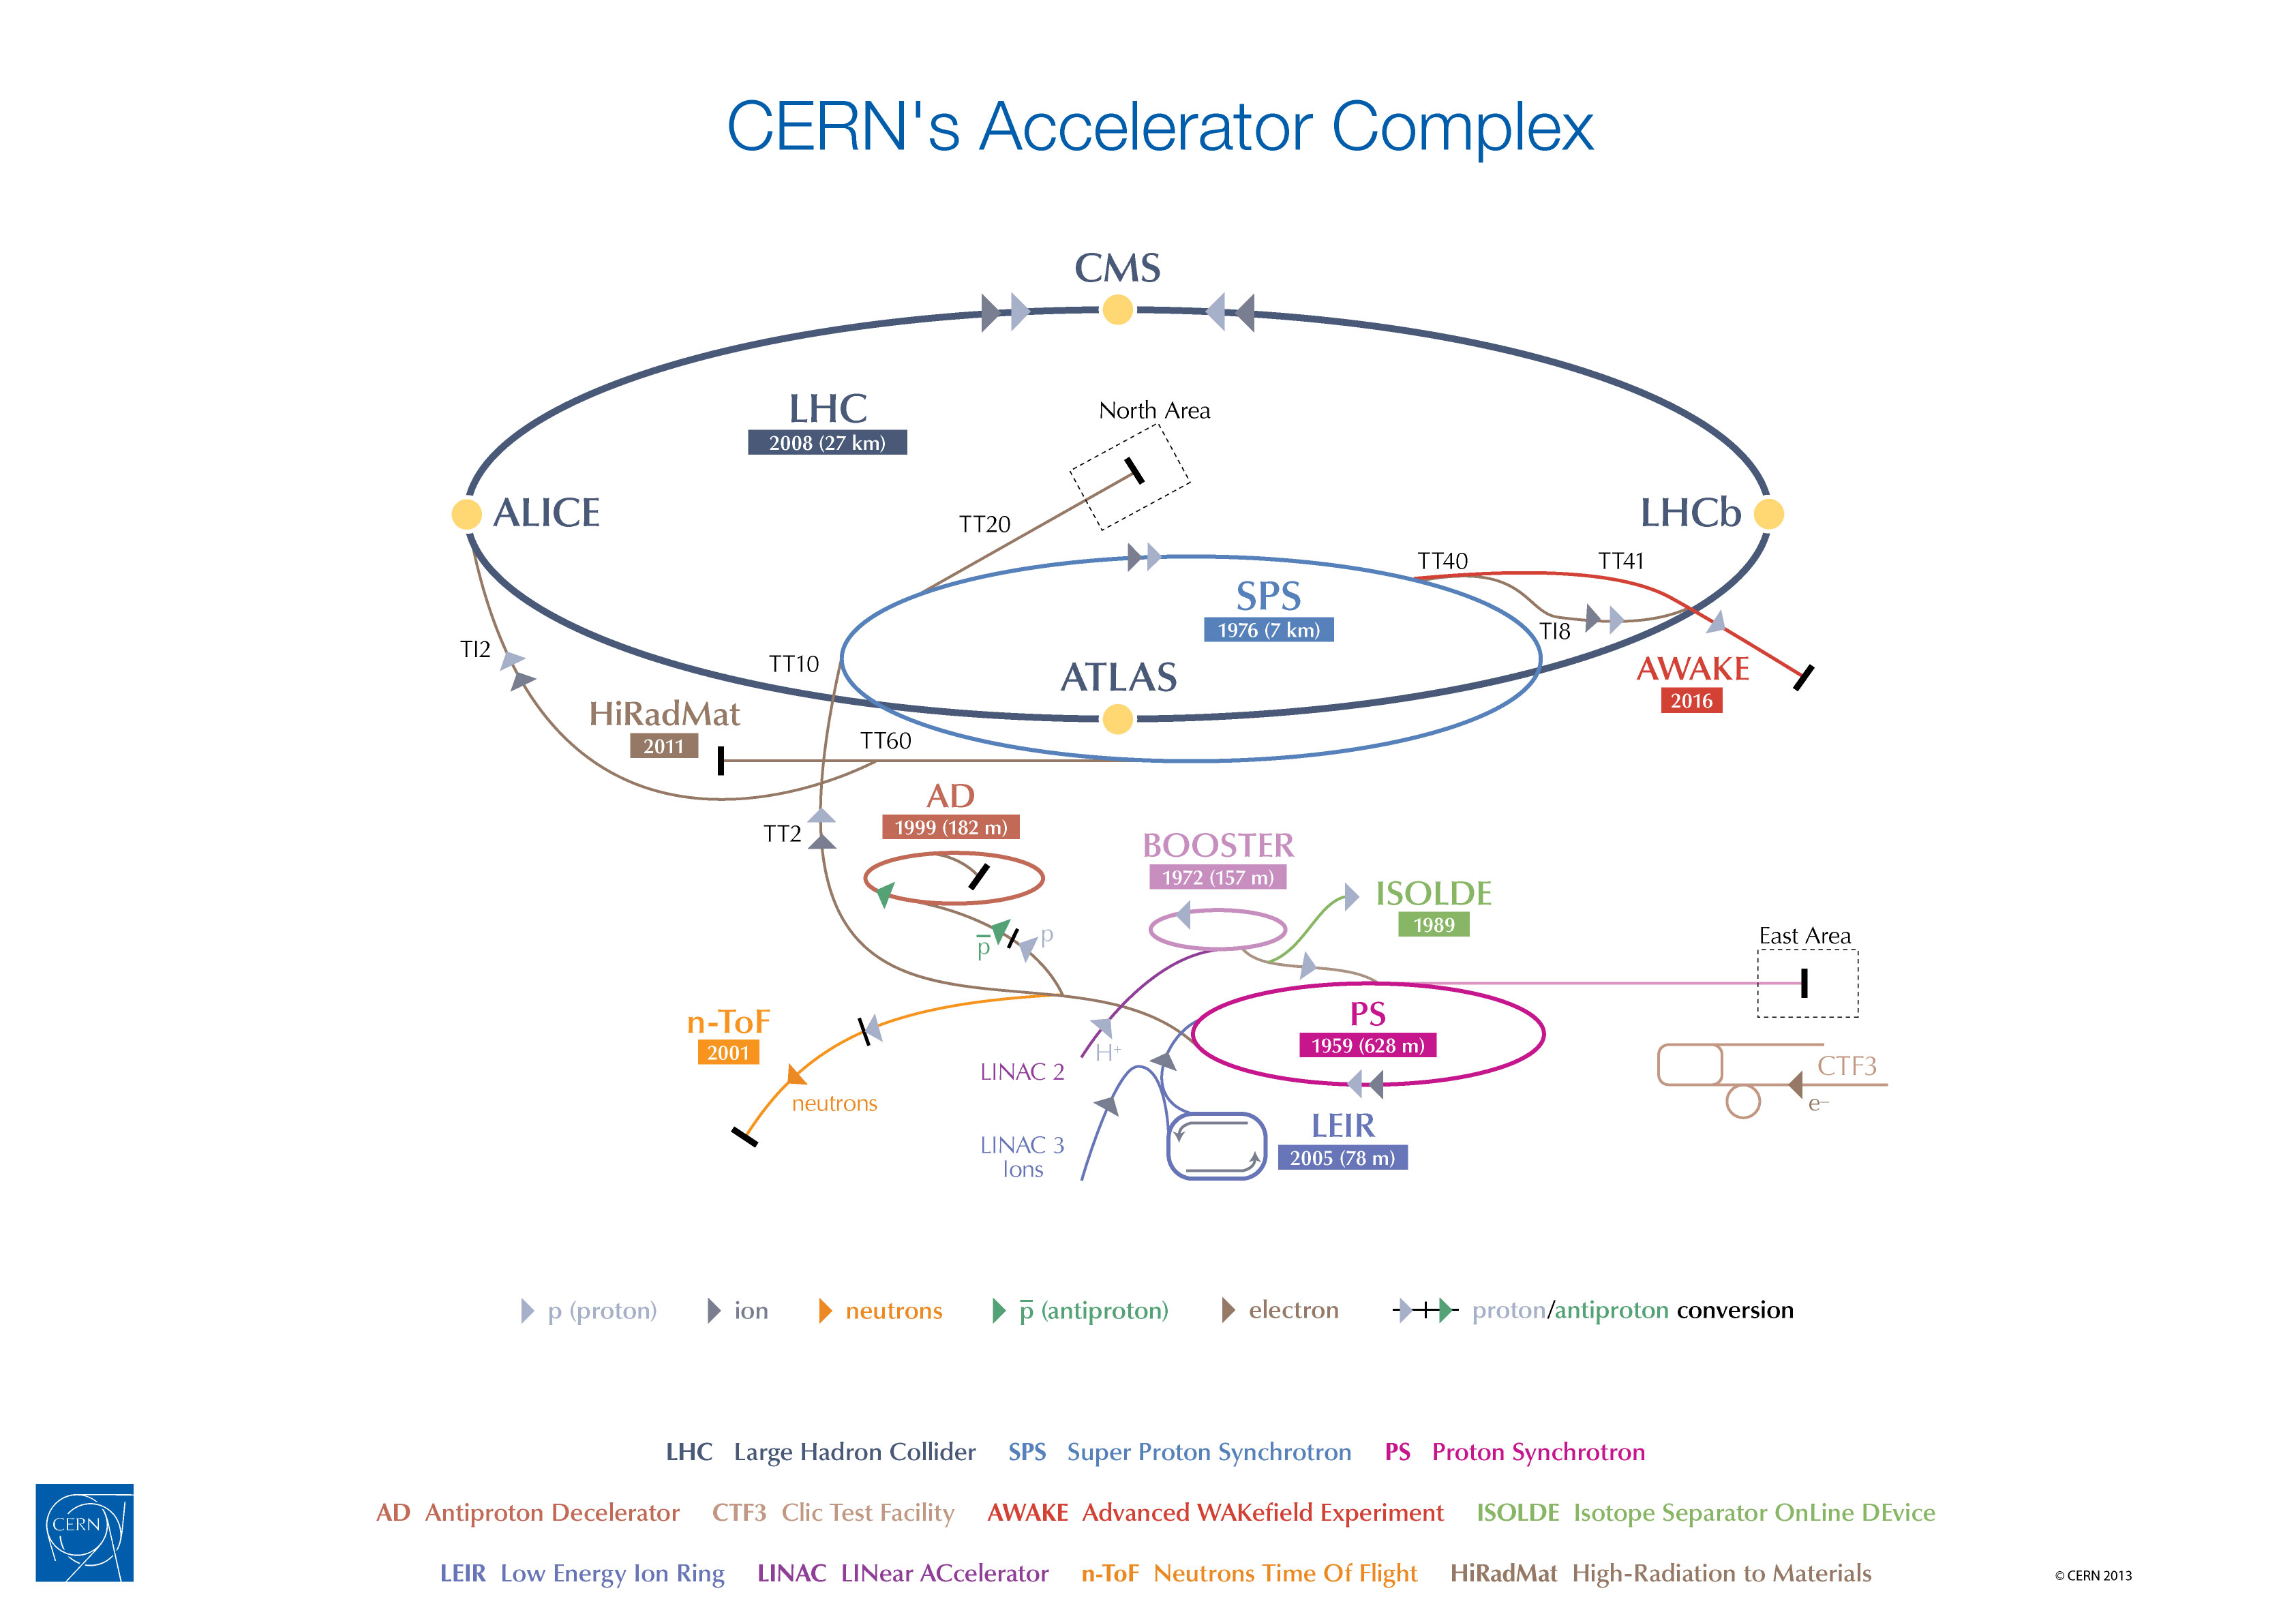
\includegraphics[scale = 0.75]{figs/Detector/LHC.jpg}
\caption{Layout of the LHC (Large Hadron COllider).}
\label{LHC}
\end{center}
\end{figure} 

The CMS and ATLAS are the two general purpose detectors to analyse the particles produced by collisions in the accelerator i.e. to cover the widest possible range of physics at the LHC,
from the search for the Higgs boson, supersymmetry (SUSY) to extra dimensions. How a prototype detector shapes into a real detector can be seen in comparison to a real detector at LHC, so we discuss below, CMS in this context.
\subsection{CMS}
The CMS (Compact Muon Solenoid) detector  is 21 m long, 15 m wide and 15 m high, shown in Figure \ref{CMS}. It is built around a huge solenoid magnet. A cylindrical coil of superconducting cable generates a magnetic field of 4 Tesla. The magnetic field is confined by a steel ``yoke'' that forms the bulk of the detector's weight of 12,500 tonnes. 

\begin{figure}[h!]
\begin{center} 
\includegraphics[scale = 0.85]{figs/Detector/CMS1.jpg}
\caption{Overview of the CMS (Compact Muon Solenoid) Detector .}
\label{CMS}
\end{center}
\end{figure}

 \begin{itemize}
\item
The particles produced from the collisions at LHC, first pass through a tracker which is made up of silicon entirely. It is a cylinder of 6m and a diameter of 2.6m. It tracks their positions and is helpful in measuring their momentum. There are calorimeters outside the tracker that measure the energy of particles. In measuring the momentum, the tracker should interfere with the particles as little as possible, whereas the calorimeters are specifically designed to stop the particles in their tracks.
 \item
The Electromagnetic Calorimeter (ECAL) is made of lead tungstate (PbWO$_{4}$) which is a very dense material that produces light when a particle hits on it. The energy of the produced photons and electrons is measured by using silicon avalanche photodiodes in the barrel and cacuum photo diodes in the endcaps. The electromagnetic calorimeter comprises of 61200 lead tungstate crystals mounted in the central barrel part and 7324 crystals in each of the two endcaps. Lead tungstate scintillating crystals were chosen because of their short radiation length \footnote{Radiation length describes the longitudinal shower development. It is a scaling variable for the probability of occurrence of bremsstrahlung, pair production and for the variance of the angle of multiple scattering. The characteristic amount of matter traversed for these related interactions is called the radiation length.} ($X_{0} = 0.89cm$) and
small Moli$\acute{e}$re (2.2 cm) radius \footnote{ A characteristic constant of a  material describing its transverse dimensions of the electromagnetic showers which are initiated by an incident high energy electron or photon.}, in order to stop all
electrons and photons within a minimal depth of the material.
This enabled the CMS collaboration to build a compact calorimeter within the solenoid.

\item
The Hadron Calorimeter (HCAL) is designed to detect any particle made up of quarks (the basic building blocks of protons and neutrons).Hadronic barrel (HB) and hadronic endcap (HE) calorimeters are sampling calorimeters with 50mm thick copper (selected because of its density) absorber plates which are interleaved with 4mm scintillator sheets. HB is made of two 4.4m length half-barrels, and HE has two large structures, situated at each end of the barrel detector and within the region of high magnetic field. Hadronic forward (HF) calorimeter are two in number and are situated at each extreme of the CMS
detector. It is made of steel absorbing plates and quartz fibers are inserted into
them. The passage of charged particles through the quartz fibers produces Cerenkov
light signals, which are used to measure the energy of the jets.

 \item
The Superconducting magnet is 13m long and 6m in diameter, and its refrigerated superconducting
niobium-titanium coils, cooled at -270$^{\circ}$C, produces a magnetic field of 4 Teslas. This intense solenoidal field is the main key to design the experiment as it is responsible for the compactness and cylindrical symmetry of the detector. The size of the magnet allows the tracker and calorimeters to be placed inside its coil, resulting in an overall compact detector. The magnetic field is obtained by a solenoid because  with the field parallel to
the beam  the bending of the muon tracks is in the transverse plane and thus making the measurement of momenta possible.

\item
As the name suggests CMS is also designed to detect muons. The outer part of the detector is the  magnet ``return yoke'', which confines and guides the magnetic field.  The four layers of detectors are interleaved with the iron  which also provides the detector's support structure. CMS was designed in fifteen separate sections or ``slices'' that were built on the surface and lowered down ready-made into the cavern. 
\end{itemize}

The basic structure of a prototype detector forms the basis for the conctruction of any real detector. There can be some changes in the design of the detector according to the needs of the aim of the experiment to be carried out with the detector.
The various detectors of the LHC have different aims which are given below in a brief way :
\begin{itemize}
\item  
The $\bf{ATLAS}$ (A Toroidal LHC Apparatus) detector shown in Figure \ref{ATLAS} is searching for new discoveries in the head-on collisions of protons with an extraordinarily high energy. The objective is to observe the phenomena that involve highly massive particles which were not observable using earlier lower-energy accelerators and the particles that could make up dark matter. It has six different detecting subsystems that identify particles and measure their momenta and energy.
 
\begin{figure}[h!]
\begin{center} 
\includegraphics[scale = 0.30]{figs/Detector/ATLASF.jpg}
\caption{Overview of the ATLAS (A Toroidal LHC Apparatus) Detector.}
\label{ATLAS}
\end{center}
\end{figure}
\item

The $\bf{ALICE}$ (A Large Ion Collider Experiment) detector shown in Figure \ref{ALICE}(a) is a heavy-ion detector which focuses on QCD. It aims to collide lead ions to recreate the conditions just after the Big Bang under laboratory conditions. It is designed to study a state of matter known as quark-gluon plasma, which is believed to have existed soon after the Big Bang. The ALICE collaboration plans to study the quark-gluon plasma as it expands and cools, observing how it progressively gives rise to the particles that constitute the matter of our Universe today.

\begin{figure}[h!]
\begin{center} 
\includegraphics[scale = 0.40]{figs/Detector/alice.jpg}%
\includegraphics[scale = 0.50]{figs/Detector/LHCb.jpg}

\caption{(a) Overview of the ALICE (A Large Ion Collider Experiment) Detector. (b)Overview of the LHCb (Large Hadron Collider beauty) Detector.}
\label{ALICE}
\end{center}
\end{figure}

\item
The $\bf{LHCb}$ (Large Hadron Collider beauty) experiment Figure \ref{ALICE}(b) will investigate the slight differences between matter and antimatter by studying a type of particle called the beauty or b quark. It will help us to understand why the Universe appears to be composed almost entirely of matter and not the antimatter. The LHCb experiment uses a series of sub-detectors to detect mainly forward particles istead of surrounding the entire collision point with an enclosed detector. An abundance of different types of quark will be created by the LHC before they decay quickly into other forms. To catch the b-quarks, LHCb has developed sophisticated movable tracking detectors close to the path of the beams circling in the LHC. It is also dedicated to precision measurements of CP violation.


\item
The $\bf{LHCf}$ (Large Hadron Collider forward) uses forward particles created inside the LHC as a source to simulate cosmic rays in laboratory conditions. Cosmic rays are naturally occurring charged particles from outer space that constantly bombard the Earth's atmosphere. They collide with nuclei in the upper atmosphere, leading to a cascade of particles that reaches ground level. LHCf will study the collisions inside the LHC which cause similar cascades of particles and it will to interpret large-scale cosmic-ray experiments.

\item
The  $\bf{TOTEM}$ (TOTal Elastic and diffractive cross section Measurement) studies forward particles to focus on physics that is not accessible to the general-purpose experiments. It will measure the total pp cross-section in a luminosity-independent method and study elastic and diffractive scattering at the LHC. TOTEM will also complement the results obtained by the CMS detector and by the other LHC experiments overall.

\end{itemize}
\end{comment}
